\chapter{Ejercicio 2.3}

\section{Varias figuras con el paquete \texttt{subcaption}}
Como podemos ver en la Figura \ref{fig:matematicos} a Gauss, en concreto en la subfigura \ref{subfig:gauss}.

\begin{figure}[h]
    \centering
    \begin{subfigure}[t]{.24\linewidth} 
    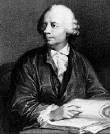
\includegraphics[height=4cm]{euler}
    \caption{Euler}\label{subfig:euler}
    \end{subfigure}
    \begin{subfigure}[t]{.24\linewidth} 
    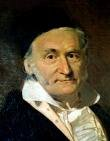
\includegraphics[height=4cm]{gauss}
    \caption{Gauss}\label{subfig:gauss}
    \end{subfigure}
    \begin{subfigure}[t]{.24\linewidth} 
    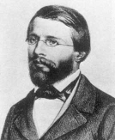
\includegraphics[height=4cm]{riemann}
    \caption{Riemann}\label{subfig:riemann}
    \end{subfigure}
    \begin{subfigure}[t]{.24\linewidth} 
    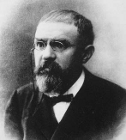
\includegraphics[height=4cm]{poincare}
    \caption{Poincare}\label{subfig:poincare}
    \end{subfigure}
    \caption{Matemáticos famosos}
    \label{fig:matematicos}
\end{figure}

Más sobre Euler en \cite{EulerWiki}.

\section{Alicia y la oruga}

La oruga y Alicia se estuvieron mirando un rato en silencio: por fin la Oruga se sacó la pipa de la boca, y se dirigió a la niña en voz lánguida y adormilada.

-¿Quién eres tú? -dijo la Oruga

No era una forma demasiado alentadora de empezar una conversación. Alicia contestó un poco intimidada:

-Apenas sé, señora, lo que soy en este momento\ldots Sí sé quién era al levantarme esta mañana, pero creo que he cambiado varias veces desde entonces.

-¿Qué quieres decir con esto? -preguntó la Oruga con severidad-. ¡A ver si te aclaras contigo misma!

\begin{wrapfigure}[16]{R}{0.30\textwidth}
  \begin{center}
    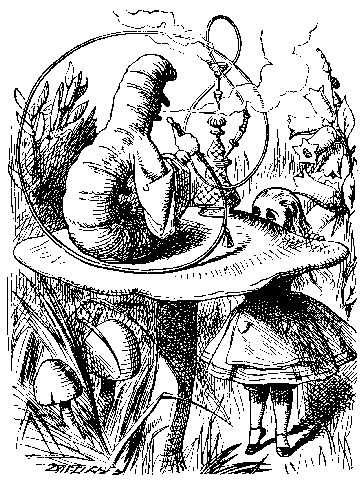
\includegraphics[width=0.30\textwidth]{oruga}
  \end{center}
  \caption{Alicia conversa con la oruga}
\end{wrapfigure}

-Temo que no puedo aclarar nada conmigo misma, señora -dijo Alicia-, porque no soy yo misma, ya lo ve.

-No veo nada -protestó la Oruga.

-Temo que no podré explicarlo con más claridad -insistió Alicia con voz amable-, porque para empezar ni siquiera lo entiendo yo misma, y eso de cambiar tantas veces de estatura en un solo día resulta bastante desconcertante.

-No resulta nada -replicó la Oruga.

-Bueno, quizás usted no haya sentido hasta ahora nada parecido -dijo Alicia-, pero cuando se convierta en crisálida, cosa que ocurrirá cualquier día, y después en mariposa, me parece que todo le parecerá un poco raro, ¿no cree?

-Ni pizca -declaró la Oruga

-Bueno,  quizá los sentimientos de usted sean distintos a los míos, porque le aseguro que a mi me parecería muy raro.

-¡A ti! -dijo la Oruga con desprecio-. ¿Quién eres tú?

Con lo cual volvían al principio de la conversación.